%!TEX root = main.tex

\section{Introduction}
\label{sec:intro}

\begin{figure*}[ht]
	\centering
	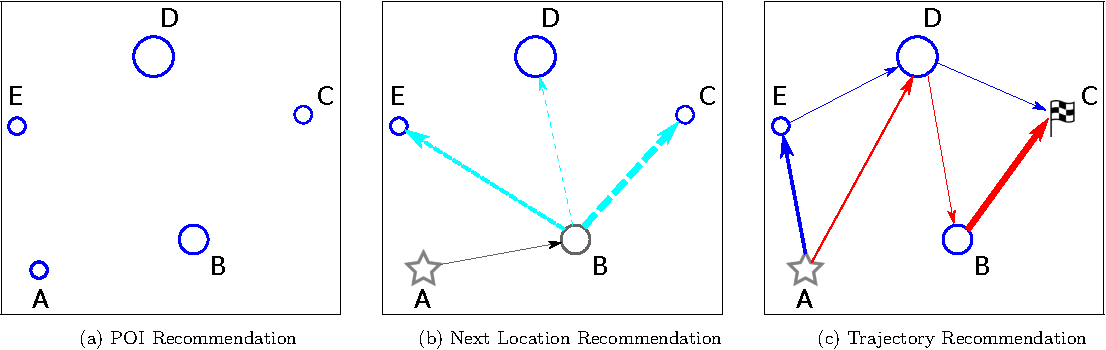
\includegraphics[width=0.7\textwidth]{fig/fig1-flavours.pdf}
	\caption{Three settings of trajectory recommendation problems: (a) POI recommendation, (b) next location recommendation, and (c) trajectory recommendation. Node size: POI score; edge width: transition score between pairs of POIs; grey: input query; star: starting location; flag: ending location. See the first four paragraphs of Section~\ref{sec:relatedwork} for details.
}
	\label{fig:threesettings}
\end{figure*}


This paper proposes a novel solution to recommend travel routes in cities.
A large amount of location traces are becoming available from ubiquitous location tracking devices.
For example FourSquare, the local search and discovery service, has 50 million monthly users who have made 8 billion check-ins~\cite{4sq}
and Flickr, the online photo-sharing site, hosts over 2 billion geo-tagged public photos~\cite{flickr}. 
Such large amounts of travel data provide new opportunities for better
travel planning traditionally done with written travel guides,
for example, choosing and ranking locations for a variety of activities from dining to recreation,
and potential new solutions to orienteering and routing problems.
Good solutions to these problems will in turn lead to better urban experiences for residents and visitors alike, and foster sharing of even more location-based behavioural data.

There are several settings of recommendation problems for locations and routes: POI recommendation,
next location recommendation, and trajectory recommendation. This is described in more detail in
Section~\ref{sec:relatedwork}, and we refer the reader to a number of recent
surveys~\cite{bao2015recommendations,zheng2015trajectory,zheng2014urban}
for general overviews of the area. %There are two notable gaps 
We note, however, that two desired qualities are still 
missing from the current solutions to trajectory recommendation. 
The first is principled method to jointly learn POI ranking, a prediction problem, 
and optimize for route creation, a planning problem. 
The second is a unified way to incorporate various features 
such as local, time, distance, user profile, social interactions, 
as they tend to get specialized and separate treatments. 
This work aims to address these challenges. %bridge these gaps. 

We propose a novel way to learn point and route preferences jointly.
Our solution consists of several parts.
We propose a learning to rank formulation to capture the preference of POIs given the starting and ending points of a trajectory (Section~\ref{sec:method}).
We model pair-wise transition patterns between POIs by factorising the transition likelihoods along five different types of location properties,
which alleviates data sparsity between each pair of POIs and allows POIs of the same type and neighbourhood to share parameters.
We combine the results of point and transition ranking using Markov chain inference and route planning techniques (Section~\ref{sec:recommendation}). We further propose a novel way to jointly learn point and transition scores with a Structured Support Vector Machine (StructuredSVM). In Section~\ref{sec:experiment},
we evaluate the proposed algorithms on photo trajectories in five different cities, with a traditional metric F$_1$ on POIs as well as a novel pairs-F$_1$ metric specifically designed for trajectories.

The main contributions of this work are as follows:
\begin{itemize}
\setlength{\itemsep}{-2pt}
\item We propose a novel algorithm to jointly optimise point preference and route plan.
  We find that the learning-based approaches generally out-perform heuristic route recommendation~\cite{ijcai15}. Incorporating transitions to POI ranking improves the pairs-F$_1$ metric for correct sequences of POIs, and that routing algorithms that disallow sub-tours generally out-perform Markov chain methods.
\item Our approach is feature-driven and learns from past behaviour without having to design specialised treatment for spatial, temporal and social information. It incorporates information about location, POI categories and behaviour history, and can use additional time, user, or social information if available.% as long as they are  encoded in features.
\item We show good performance compared to recent results~\cite{ijcai15}, and also quantify the contribution from the different components, such as ranking points, scoring transitions, and routing.
\item We propose a new metric to evaluate trajectories: pairs-F$_1$, which has the property of being between 0 and 1, and being 1 if and only if the recommended trajectory is exactly the same as the ground truth. Our benchmark data and results are publicly available.
\end{itemize}
